\let\negmedspace\undefined
\let\negthickspace\undefined
\documentclass[journal]{IEEEtran}
\usepackage[a5paper, margin=10mm, onecolumn]{geometry}
%\usepackage{lmodern} % Ensure lmodern is loaded for pdflatex
\usepackage{tfrupee} % Include tfrupee package

\setlength{\headheight}{1cm} % Set the height of the header box
\setlength{\headsep}{0mm}     % Set the distance between the header box and the top of the text

\usepackage{gvv-book}
\usepackage{gvv}
\usepackage{cite}
\usepackage{amsmath,amssymb,amsfonts,amsthm}
\usepackage{algorithmic}
\usepackage{graphicx}
\usepackage{textcomp}
\usepackage{xcolor}
\usepackage{txfonts}
\usepackage{listings}
\usepackage{enumitem}
\usepackage{mathtools}
\usepackage{gensymb}
\usepackage{comment}
\usepackage[breaklinks=true]{hyperref}
\usepackage{tkz-euclide} 
\usepackage{listings}
% \usepackage{gvv}                                        
\def\inputGnumericTable{}                                 
\usepackage[latin1]{inputenc}                                
\usepackage{color}                                            
\usepackage{array}                                            
\usepackage{longtable}                                       
\usepackage{calc}                                             
\usepackage{multirow}                                         
\usepackage{hhline}                                           
\usepackage{ifthen}                                           
\usepackage{lscape}
\begin{document}

\bibliographystyle{IEEEtran}
\vspace{3cm}

\title{1.3.4}
\author{EE24BTECH11002 - Agamjot Singh
}
% \maketitle
% \newpage
% \bigskip
{\let\newpage\relax\maketitle}

\renewcommand{\thefigure}{\theenumi}
\renewcommand{\thetable}{\theenumi}
\setlength{\intextsep}{10pt} % Space between text and floats

\textbf{Question:}
\newline
If $\vec{A}\brak{1,3}$, $\vec{B}\brak{-1,2}$, $\vec{C}\brak{2,5}$ and $\vec{D}\brak{x,4}$ are the vertices of a parallelogram $ABCD$, then the value of x is
\newline
\textbf{Solution:}
By definition of parallelogram, we say that the line $\vec{AD}$ is parallel to the line $\vec{BC}$. 
Therefore, the slopes of these lines must be equal.
\newline

The direction vector of $\vec{PQ}$ is defined as
\begin{align*}
	\vec{m} = \vec{Q} - \vec{P} = k\myvec{1\\m}
\end{align*}

where $m$ is the slope of $\vec{PQ}$. We also say that
\begin{align*}
	\vec{m}\equiv\myvec{1\\m}
\end{align*}

Direction vector of $\vec{m} = \vec{BC}$ is given as
\begin{align}
	\vec{m}  &= \vec{C} - \vec{B}\\
	\vec{m}  &= \myvec{2\\5}  - \myvec{-1\\2}
		 = \myvec{3\\3}\\
	\vec{m}  &\equiv \myvec{1\\1}\\
	       m &= 1	
\end{align}

So, the slope of $\vec{BC}$ is $1$, which is equal to the slope of $\vec{AD}$.
\newline
Direction vector of $\vec{m_1} = \vec{AD}$ is given as
\begin{align}
	\vec{m_1} &= \vec{D} - \vec{A}\\
	\vec{m_1} &= \myvec{x\\4} - \myvec{1\\3}
		   = \myvec{x-1\\1}\\
	\vec{m_1} &\equiv \myvec{1\\\frac{1}{x-1}}
\end{align}

By equation $\brak{7}$, we get the slope of $\vec{AD}$ is $\frac{1}{x-1}$.
\newline
By equation $\brak{4}$, we get
\begin{align}
	\frac{1}{x - 1} &= 1\\
	x &= 2
\end{align}

\begin{figure}[h!]
   \centering
   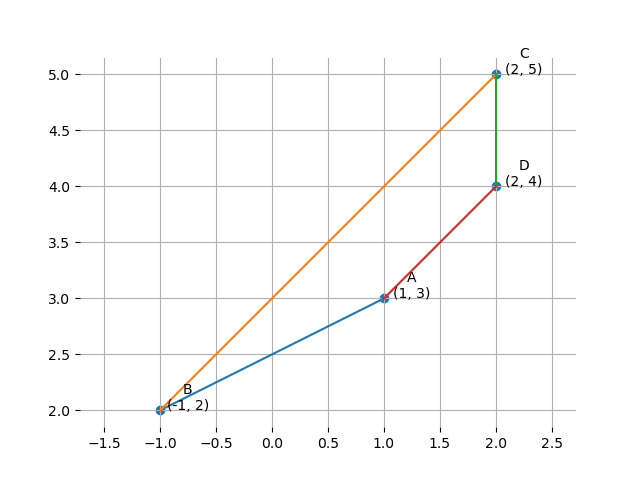
\includegraphics[width=0.7\linewidth]{figs/graph.png}
   \caption{Quadrilateral ABCD formed with given equations}
   \label{label}
\end{figure}

As we can see in the graph, the given quadrilateral formed with $x$ found in equation $\brak{9}$ is not a parallelogram.
Therefore, we conclude that there is no $x$ for which $ABCD$ is a parallelogram.

\end{document}
